% Deck for the maintained MetaG_new pipeline. Build with `make` in this folder.
% Describes production PHYSICS_VERSION 2026-10-07e and its measured performance.
% Full-panel accuracy is from the last frozen release (2026-10-01c); 07e has not been re-benchmarked.
% Previous (6 October) version: archive/MetaG_20261006.{tex,pdf}.
\documentclass[aspectratio=169,11pt]{beamer}
\usepackage[T1]{fontenc}
\usepackage[utf8]{inputenc}
\usepackage{lmodern}
\usepackage{amsmath,amssymb,booktabs,graphicx,tikz,array}
\usetikzlibrary{arrows.meta,positioning,calc}
\graphicspath{{figures/}}
\newcolumntype{L}[1]{>{\raggedright\arraybackslash}p{#1}}
\newcolumntype{R}[1]{>{\raggedleft\arraybackslash}p{#1}}
\definecolor{teal}{HTML}{087F8C}
\definecolor{ink}{HTML}{173640}
\definecolor{muted}{HTML}{617780}
\definecolor{pale}{HTML}{EDF5F6}
\definecolor{amber}{HTML}{B77818}
\definecolor{sand}{HTML}{FAF3E6}
\setbeamercolor{normal text}{fg=ink,bg=white}
\setbeamercolor{structure}{fg=teal}
\setbeamercolor{frametitle}{fg=ink}
\setbeamercolor{block title}{fg=teal,bg=white}
\setbeamercolor{block body}{fg=ink,bg=white}
\setbeamercolor{alerted text}{fg=amber}
\setbeamerfont{frametitle}{size=\Large,series=\bfseries}
\setbeamerfont{block title}{series=\bfseries}
\setbeamertemplate{navigation symbols}{}
\setbeamertemplate{itemize item}{\color{teal}\small$\bullet$}
\setbeamertemplate{frametitle}{\vspace{.28cm}\insertframetitle\par\vspace{.12cm}\textcolor{teal}{\rule{\linewidth}{.6pt}}}
\setbeamertemplate{footline}{\hspace{.45cm}\color{muted}\scriptsize MetaG\hfill Pipeline and performance\hfill 7 October 2026\quad\insertframenumber\hspace{.45cm}\vspace{.20cm}}
\setbeamersize{text margin left=.65cm,text margin right=.65cm}
\newcommand{\src}[1]{\vfill{\tiny\color{muted}Evidence: #1\par}}
\newcommand{\messagebox}[1]{\par\vspace{.22cm}{\small\color{muted}#1\par}}
\newcommand{\dg}{\Delta_r G^{\prime\circ}}
\newcommand{\unit}{\mathrm{kJ\,mol^{-1}}}
\newcommand{\gap}{\vspace{.18cm}}
\newcommand{\sectionslide}[2]{\begin{frame}[plain]\vfill{\color{teal}\large #1}\par\vspace{.25cm}{\LARGE\bfseries #2}\par\vfill\end{frame}}
\title{MetaG}
\subtitle{From molecular structure to metabolic reaction Gibbs energy}
\author{Ray Zhu}
\date{7 October 2026}
\begin{document}

% ---------------------------------------------------------------------------
\begin{frame}[plain]
\vspace{.35cm}
{\color{teal}\large Metabolic reaction thermodynamics}\par\vspace{.45cm}
{\Huge\bfseries MetaG}\par\vspace{.20cm}
{\LARGE From molecular structure to\\metabolic reaction Gibbs energy}\par\vspace{.45cm}
{\large Pipeline and benchmark performance}\par\vspace{.6cm}
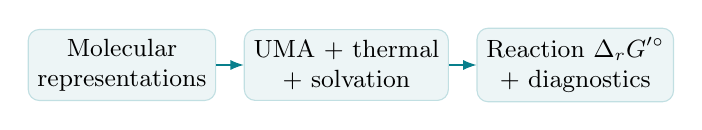
\begin{tikzpicture}[node distance=.35cm, every node/.style={rounded corners,fill=pale,draw=teal!25,minimum height=.9cm,font=\small,align=center}]
\node (a) {Molecular\\representations};
\node[right=of a] (b) {UMA + thermal\\+ solvation};
\node[right=of b] (c) {Reaction $\dg$\\+ diagnostics};
\draw[-{Latex},teal] (a)--(b);\draw[-{Latex},teal] (b)--(c);
\end{tikzpicture}
\vfill{\color{muted}Ray Zhu\hfill Collaborator discussion\quad 7 October 2026}
\end{frame}

\begin{frame}{Scope and thermodynamic convention}
\begin{columns}[T]
\column{.53\textwidth}
\begin{block}{Aim}
Use UMA as the electronic-energy core, with physically justified molecular states and thermodynamic corrections.
\end{block}
\gap
Apply the same chemical rules to unseen ModelSEED reactions. Every result should explain its representation, energy terms, and limitations.
\column{.43\textwidth}
\textbf{Target conditions}\gap
\begin{itemize}\item $T=298.15$ K; pH 7\item Ionic strength $I=0$\item No Mg-binding contribution\item Solutes at 1 M; pure liquid water\end{itemize}
\end{columns}
\messagebox{For metabolite concentrations, a separate reaction-quotient term is needed: $\Delta_rG^\prime=\dg+RT\ln Q^\prime$.}
\src{README; pipeline.py (CONDITIONS); assembly.py. Conditions are fixed in the current code.}
\end{frame}

\begin{frame}{Where empirical information enters}
\begin{columns}[T]
\column{.31\textwidth}\begin{block}{Electronic model}\small UMA is trained on quantum-chemical data (OMol25). It predicts energies and forces for specified geometries, charge, and spin.\end{block}
\column{.31\textwidth}\begin{block}{Thermodynamic model}\small Conformers, thermal corrections, solvation, chemical states, standard states, and stoichiometry convert those energies into $\dg$.\end{block}
\column{.31\textwidth}\begin{block}{Empirical constants}\small pKa references, the experimental hydration free energy of water, and carbonyl hydration constants. openTECR is used for evaluation and interval calibration.\end{block}
\end{columns}
\gap
\textbf{No openTECR reaction-energy offset is fitted in the point estimate.}
\gap
Routing rules were developed with openTECR in view, so openTECR scores are development results, not independent validation.
\src{production\_policy.py; pka\_transform.py; aldehyde\_hydration.py; config.py (ANCHOR\_CORRECT off).}
\end{frame}

\begin{frame}{Pipeline}
\centering
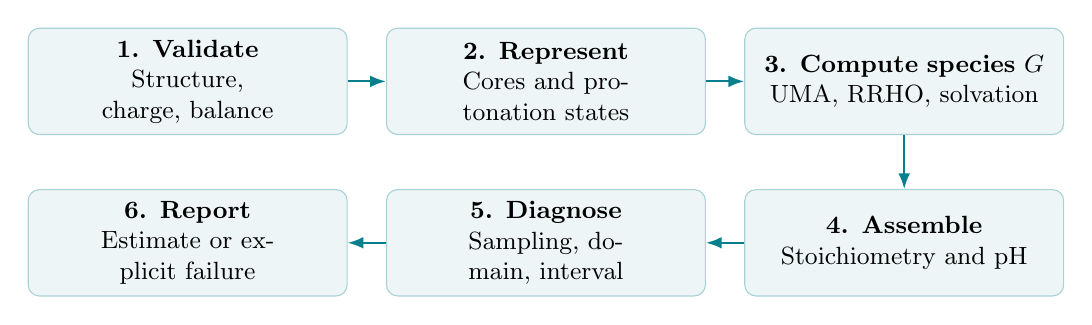
\begin{tikzpicture}[x=1cm,y=1cm,
 card/.style={draw=teal!35,fill=pale,rounded corners,minimum width=4.05cm,minimum height=1.35cm,text width=3.65cm,align=center,font=\small},
 arr/.style={-{Latex[length=2mm]},thick,teal}]
\node[card] (a) at (0,0) {\textbf{1. Validate}\\Structure, charge, balance};
\node[card] (b) at (4.55,0) {\textbf{2. Represent}\\Cores and protonation states};
\node[card] (c) at (9.10,0) {\textbf{3. Compute species $G$}\\UMA, RRHO, solvation};
\node[card] (f) at (0,-2.05) {\textbf{6. Report}\\Estimate or explicit failure};
\node[card] (e) at (4.55,-2.05) {\textbf{5. Diagnose}\\Sampling, domain, interval};
\node[card] (d) at (9.10,-2.05) {\textbf{4. Assemble}\\Stoichiometry and pH};
\draw[arr] (a)--(b);\draw[arr] (b)--(c);\draw[arr] (c)--(d);\draw[arr] (d)--(e);\draw[arr] (e)--(f);
\end{tikzpicture}
\gap
\gap\small Experimental labels enter only evaluation and uncertainty calibration, after point-energy assembly.
\src{routing/planner.py; energetics/; assembly.py; pipeline.py; uncertainty.py.}
\end{frame}

\begin{frame}{Exact composition of the reaction energy}
\vspace{-.2cm}
\[
 \dg=\sum_i \nu_i\,G_i^{\rm eff}\;+\;n_{\rm H^+}\,G_{\rm H^+}\;+\;\sum_{j\in\text{sites}} s_j\,m_j\,\Delta G_j^{\rm pKa}
\]
\vspace{-.15cm}\small
\renewcommand{\arraystretch}{1.55}
\begin{tabular}{@{}L{3.1cm}l@{}}
Solute (core or full) & $G_i=-RT\ln\sum_k e^{-(E^{\rm UMA}_k+G^{\rm RRHO}_k+\Delta G^{\rm ALPB}_k)/RT}\;+\;RT\ln 24.46$\\
Carbonyl hydration & $G_i^{\rm eff}=-RT\ln\big[e^{-G_i/RT}+\sum_S e^{-(G_S-n_S G_{\rm w})/RT}\big]$\\
Liquid water & $G_{\rm w}=E^{\rm UMA}+G^{\rm RRHO}+\Delta G^{\rm exp}_{\rm hyd}+RT\ln 55.34+RT\ln 24.46$\\
Proton at pH 7 & $G_{\rm H^+}=-26.3-1104.5-RT\ln10\cdot\mathrm{pH}=-1170.8$\\
pKa site $j$ & $\Delta G_j^{\rm pKa}=-RT\ln10\;\log_{10}\big(1+10^{\pm(\mathrm{pH}-pK_{a,j})}\big)$\\
\end{tabular}\par\vspace{.1cm}
\scriptsize
$k$: validated conformer minima. $S$: distinct hydrates with $n_S$ waters. $s_j=\pm1$ product/reactant, $m_j$ multiplicity, $+$ acid / $-$ base.
$RT\ln24.46=7.93$ (1 atm$\rightarrow$1 M); $RT\ln55.34=9.96$; $\Delta G^{\rm exp}_{\rm hyd}=-26.4$ kJ/mol.
$G^{\rm RRHO}$: ZPE + ideal-gas terms at 1 atm, exact UMA Hessian, 50 cm$^{-1}$ floor, detected linearity and symmetry number.
\textbf{Off by default:} class anchors, SMD correction, hydro-lyase water patch, ring--chain forms, qRRHO.
\src{assembly.assemble\_reaction; pipeline.py (G\_HPLUS, STD\_STATE\_KJ, water\_ref\_G); protonation.site\_free\_energy; aldehyde\_hydration.mixture\_G\_states; config.py.}
\end{frame}

\begin{frame}{Conformers and thermal ensemble}
\begin{columns}[T]
\column{.48\textwidth}\textbf{Sampling}\gap
\begin{itemize}
\item ETKDG/MMFF pool, ranked by UMA single points
\item Lowest candidates relaxed with UMA; ALPB at the same geometry
\item Batches added until the ensemble $G$ plateaus
\item Independent seed sequences available for convergence checks
\end{itemize}
\column{.48\textwidth}\textbf{Minimum validation}\gap
\begin{itemize}
\item Every sampled candidate must be a validated minimum
\item Imaginary modes: retighten, then follow the mode both ways
\item Retry with 1200 optimization steps if unresolved
\item Still unresolved, or $>64$ candidates: species fails explicitly
\end{itemize}
\end{columns}
\messagebox{The within-run spread $U_{\rm samp}$ does not bound unsampled basins; flexible molecules need independent-seed checks.}
\src{energetics/sampling.py; energetics/thermal\_ensemble.py; pipeline.py (THERMAL\_VALIDATION\_MAX, THERMAL\_RETRY\_STEPS).}
\end{frame}

\begin{frame}{Checks on every species}
\begin{columns}[T]
\column{.48\textwidth}\textbf{Identity}\gap
\begin{itemize}
\item Connectivity and specified stereochemistry verified after every relaxation
\item Explicit-water clusters: solute identity and intact waters
\item Solvation, RRHO and electronic energy from the same geometry
\end{itemize}
\column{.48\textwidth}\textbf{Failure reporting}\gap
\begin{itemize}
\item Unsupported chemistry is refused, not approximated
\item No-estimates state the cause: time budget, unresolved minimum, energy failure, quarantined pKa
\item Charge-closure and $|\dg|$ sanity guards fail closed
\end{itemize}
\end{columns}
\messagebox{A result with $\dg$ = null is a failed estimate, not zero energy.}
\src{energetics/conformers.py (same\_stereochemistry); pipeline.score\_reaction guards; \_no\_estimate.}
\end{frame}

\begin{frame}{Structural cores: CoA example}
\centering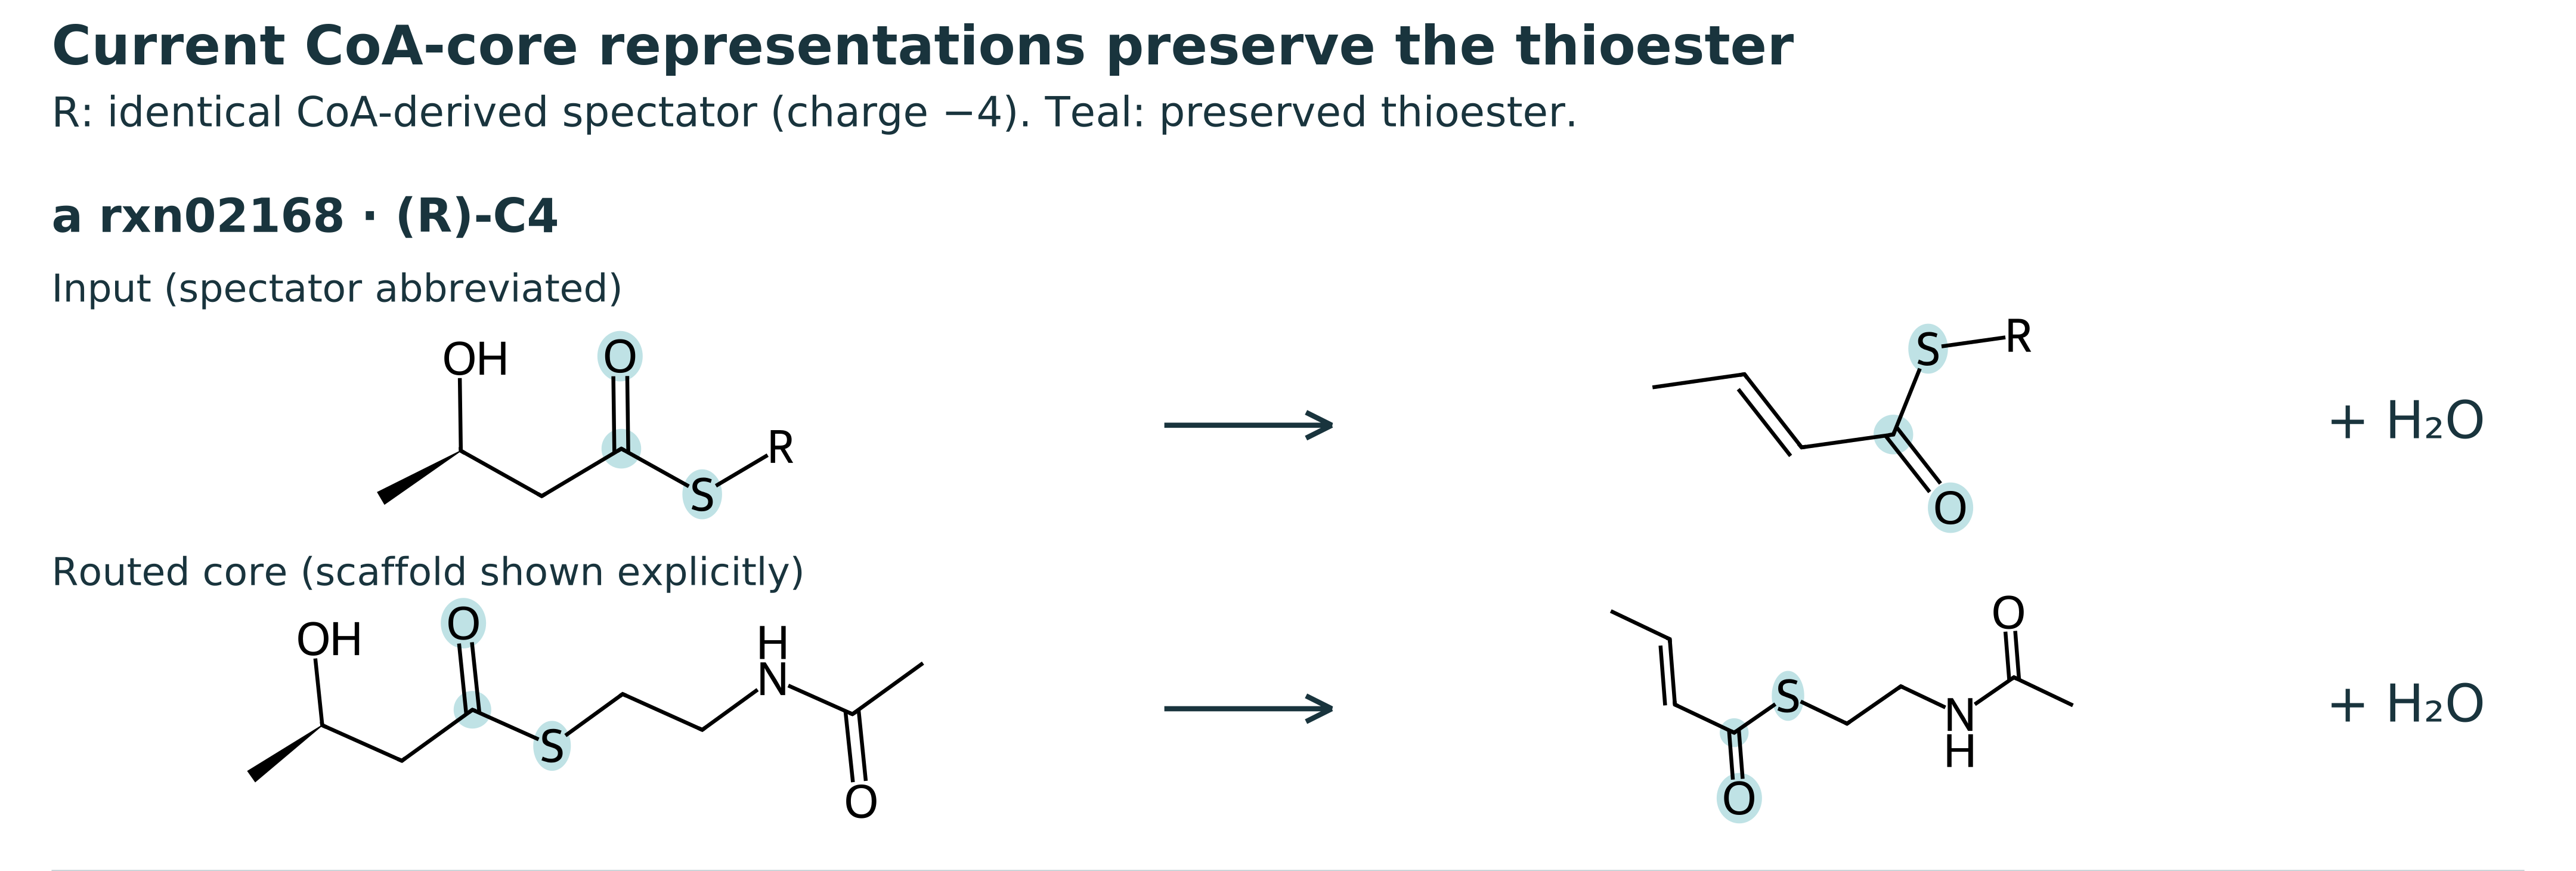
\includegraphics[width=.96\textwidth,height=4.1cm,keepaspectratio]{coa_core_example.png}
\messagebox{The CoA route retains the thioester and an amide-containing scaffold. These structures come directly from the router.}
\src{rxn02168 route; balance and spectator identity checked by make\_truncation\_figure.py.}
\end{frame}

\begin{frame}{Truncation acceptance}
\begin{columns}[T]
\column{.47\textwidth}\begin{block}{Structural guards}\small Element and charge balance\par Consistent removed fragments\par Intact rings and reactive bonds\par Preserved proton accounting\end{block}
\column{.49\textwidth}\begin{block}{Energetic check}\small Radius $R$ and $R+1$ must be different molecular models\par $|\Delta G_{R+1}-\Delta G_R|\le$ tolerance, and\par $2\sqrt{U_R^2+U_{R+1}^2}\le$ tolerance\par Otherwise: full molecule\end{block}
\end{columns}
\messagebox{This is a guard, not a convergence proof. Remaining cofactor/NTP core approximations are reported with each result.}
\src{pipeline.\_score\_trunc\_validated; routing/truncate.py; routing/cofactor\_truncate.py.}
\end{frame}

\begin{frame}{Protonation and chemical states}
\begin{columns}[T]
\column{.48\textwidth}\textbf{Protonation}\gap
\begin{itemize}
\item Reference microspecies computed in QM; pKa terms bring them to pH 7
\item Independent-site treatment of multiple sites
\item Missing pKa entries are not fabricated
\item Unsupported phosphorus environments refused; P--N ladder quarantined
\end{itemize}
\column{.48\textwidth}\textbf{Solvation and hydration}\gap
\begin{itemize}
\item Gas-phase UMA minima + ALPB solvation
\item Liquid water from experiment
\item Carbonyl hydrates as distinct species, constants from independent $K_{\rm hyd}$ data
\item Ring--chain and explicit-water paths: optional, off
\end{itemize}
\end{columns}
\messagebox{Coupled multi-site protonation needs a map from the QM microstate to measured macrostates; a sequential-pKa routine exists but is not routed.}
\src{energetics/protonation.py; pka\_transform.py; pka\_domain.py; aqueous\_states.py; docs/pka-provenance.md.}
\end{frame}

% ---------------------------------------------------------------------------
\sectionslide{Performance}{Accuracy, coverage and baselines}

\begin{frame}{Benchmark panel and reference labels}
\begin{columns}[c]
\column{.60\textwidth}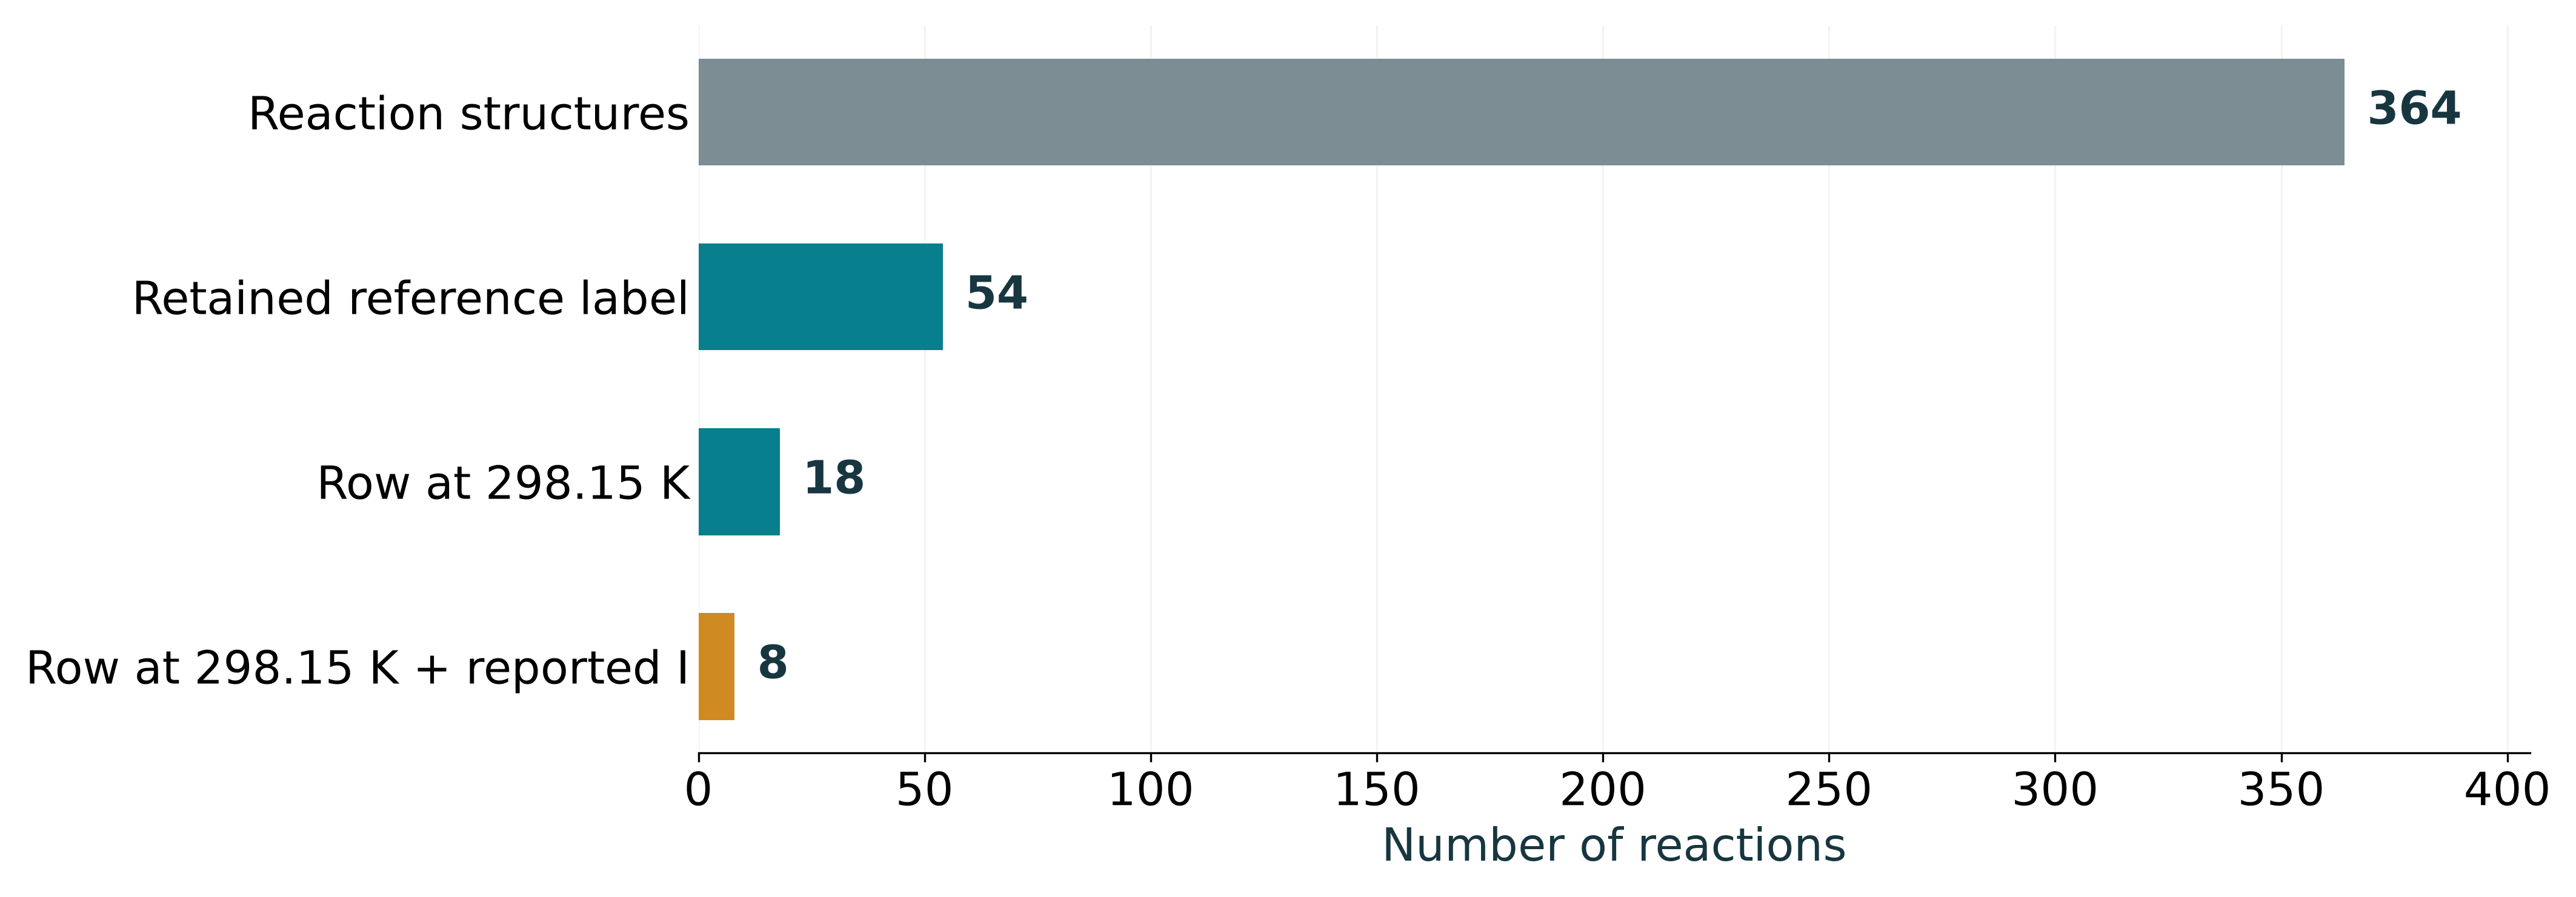
\includegraphics[width=\linewidth,height=5cm,keepaspectratio]{reference_coverage.png}
\column{.36\textwidth}\small
\textbf{364} openTECR reactions with structures; all are scored.\par\gap
\textbf{54} keep a label after strict curation; \textbf{8} have a measurement at 298.15 K with reported ionic strength.\par\gap
The full-panel numbers that follow use archived labels, whose conditions are not all resolved.
\end{columns}
\src{curated/reference\_report.json; src/metag/data/reactions\_opentecr\_std.json.}
\end{frame}

\begin{frame}{Accuracy on openTECR}
\begin{columns}[c]
\column{.52\textwidth}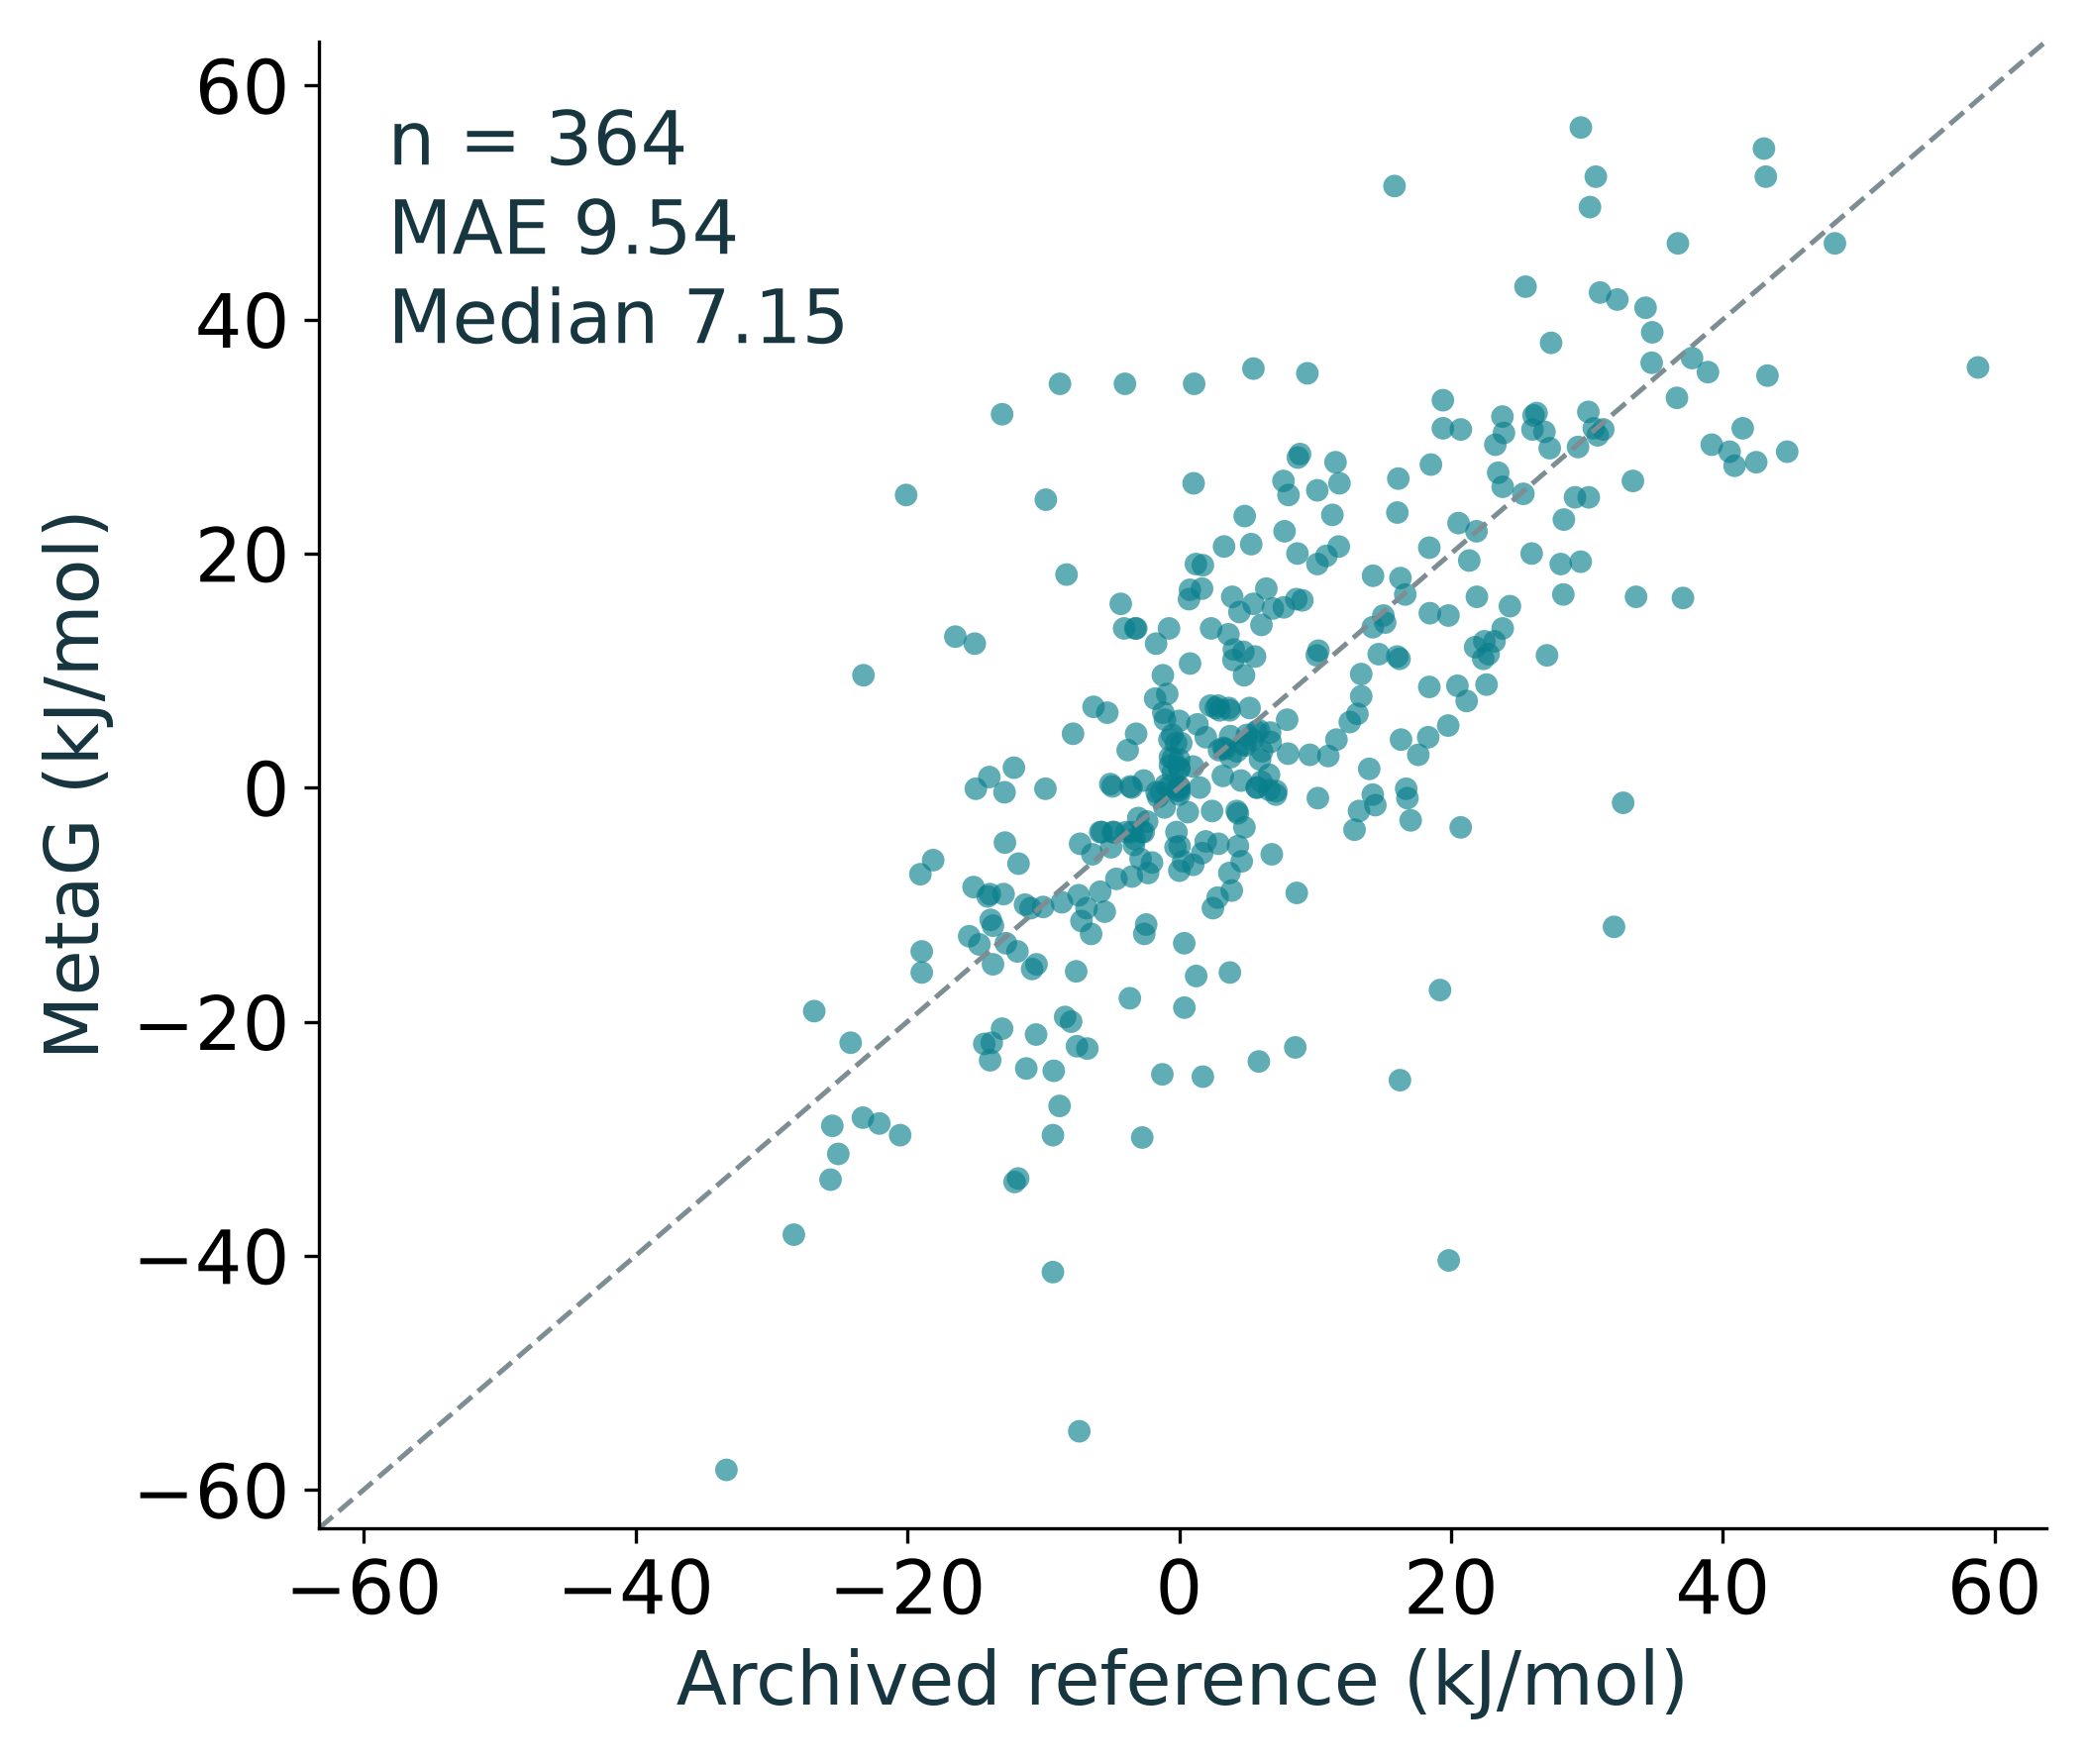
\includegraphics[width=\linewidth,height=5.25cm,keepaspectratio]{historical_accuracy.png}
\column{.44\textwidth}\small
\begin{tabular}{lr}
\toprule
Reactions scored & 364 / 364\\
MAE & 9.54 kJ/mol\\
Median absolute error & 7.15 kJ/mol\\
Errors $>$ 20 kJ/mol & 35\\
Labels inside 95\% interval & 97\%\\
Median interval half-width & 29.7 kJ/mol\\\bottomrule
\end{tabular}\par\gap
Release 2026-10-01c, archived labels. Development result: rules were chosen with this panel in view.\par\gap
The current version (07e) adds stricter validation and has not yet been re-benchmarked on the full panel.
\end{columns}
\src{artifacts/results/metag\_opentecr\_calibrated (364 records; interval coverage in-sample).}
\end{frame}

\begin{frame}{Comparison with pretrained baselines}
\centering
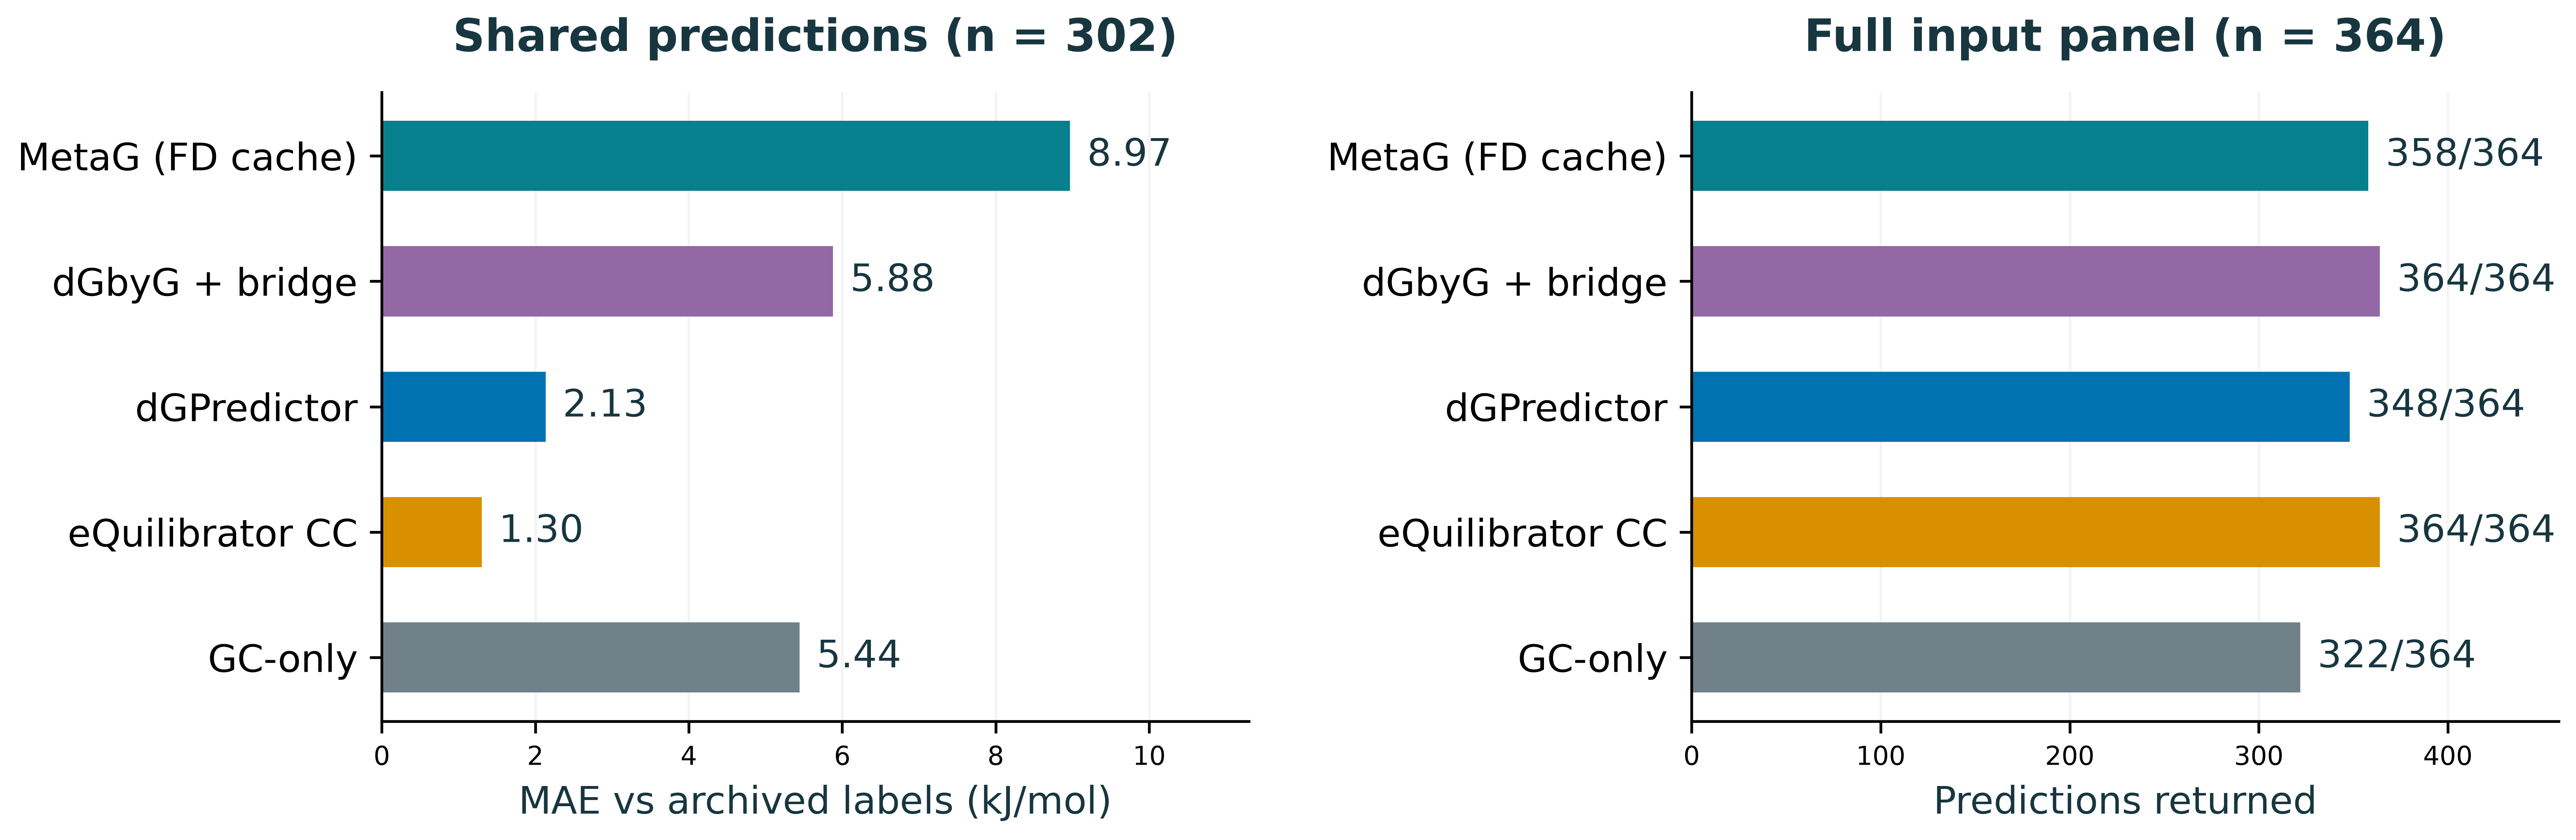
\includegraphics[width=\linewidth,height=3.8cm,keepaspectratio]{benchmark_summary.png}\par
\gap
\small 302 reactions predicted by every method; archived openTECR labels. MetaG withholds 6 phosphorus cases (4 P--N, 2 phosphonate).
\gap
The baselines are trained on TECRDB data: 148/302 shared reactions match dGbyG training reactions. This is not held-out accuracy.
\src{artifacts/benchmark/comparison; Fan et al., Cell Systems (2025), DOI: 10.1016/j.cels.2025.101393.}
\end{frame}

\begin{frame}{Strict reference conditions (small subset)}
\centering
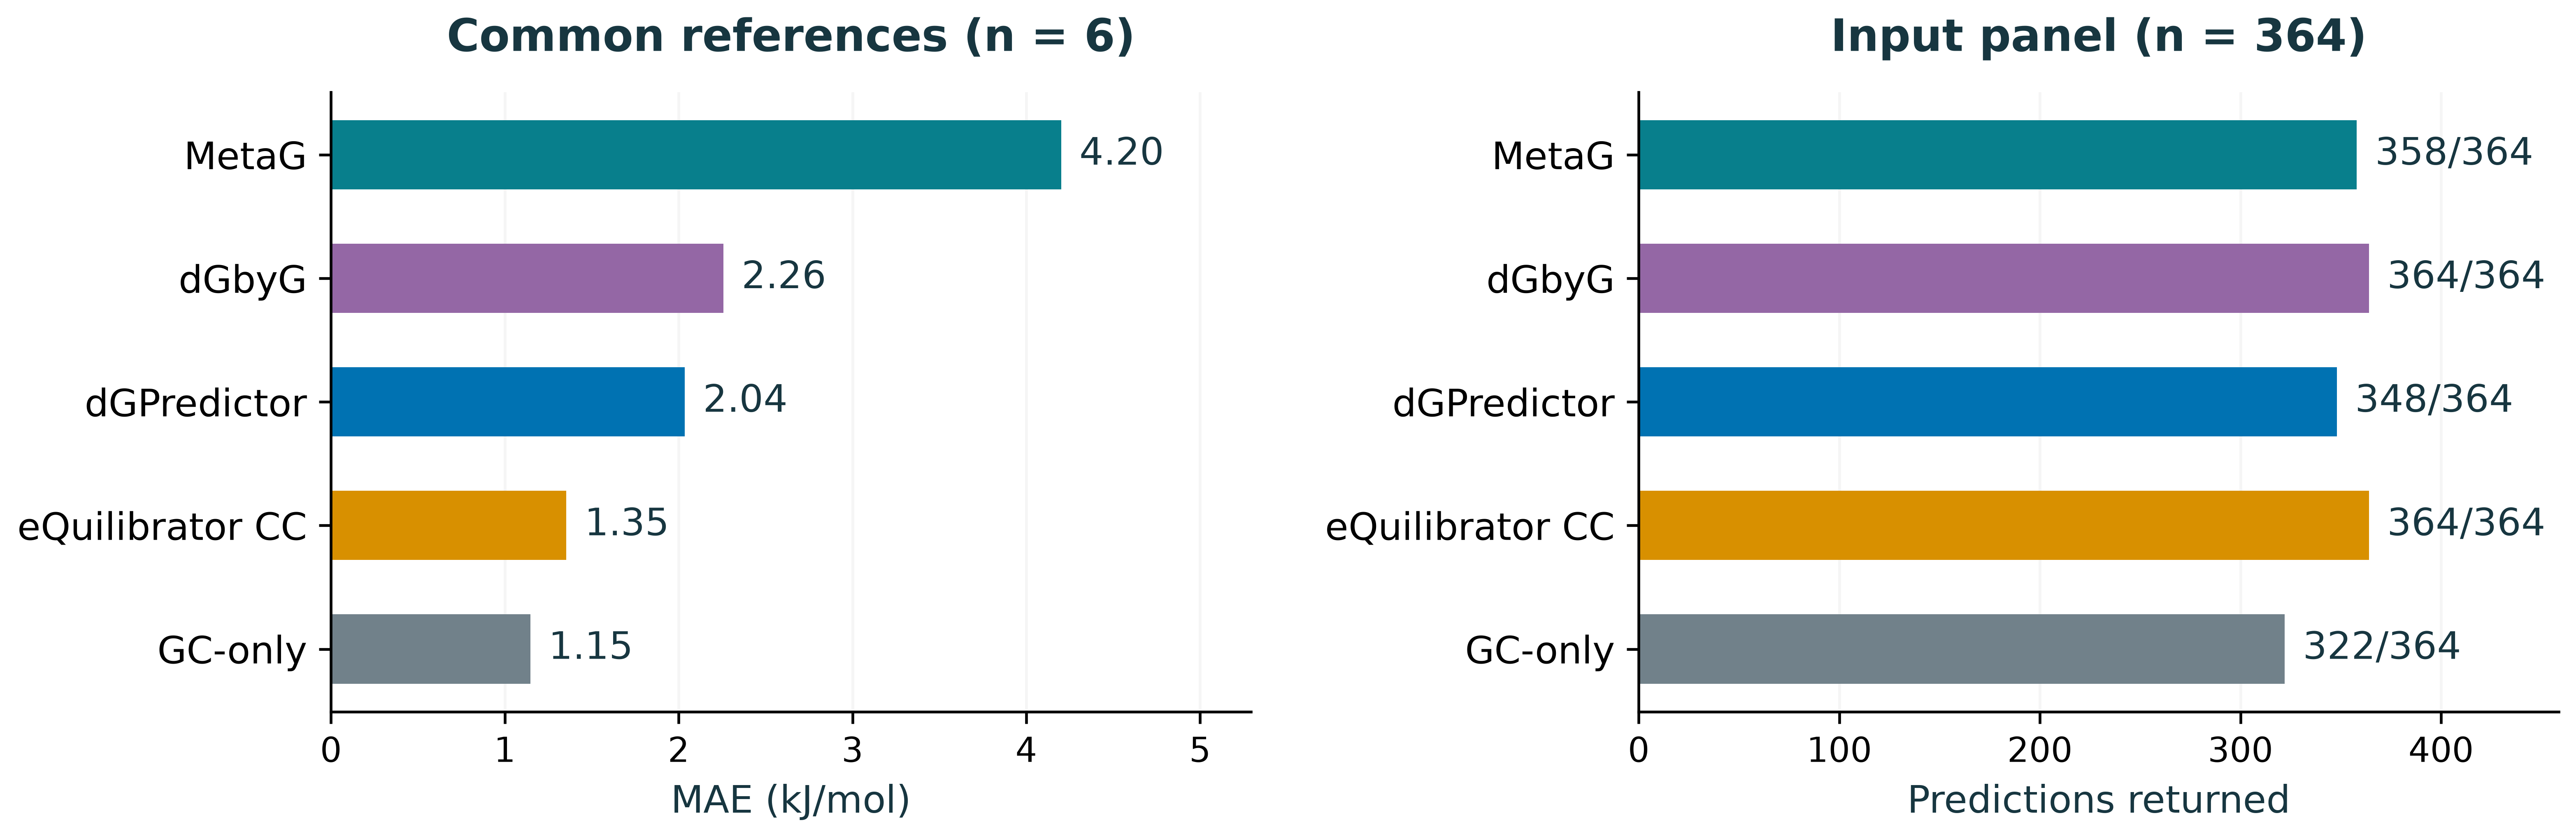
\includegraphics[width=\linewidth,height=3.8cm,keepaspectratio]{benchmark_strict_summary.png}\par
\gap
\small Eight reactions have a measurement at 298.15 K with reported ionic strength; six are supported by all methods. All six match dGbyG training reactions.
\src{artifacts/benchmark/comparison; native dGbyG I=0.25 M output excluded from the I=0 comparison.}
\end{frame}

\begin{frame}{MetaG vs held-out dGbyG on matched reactions}
\centering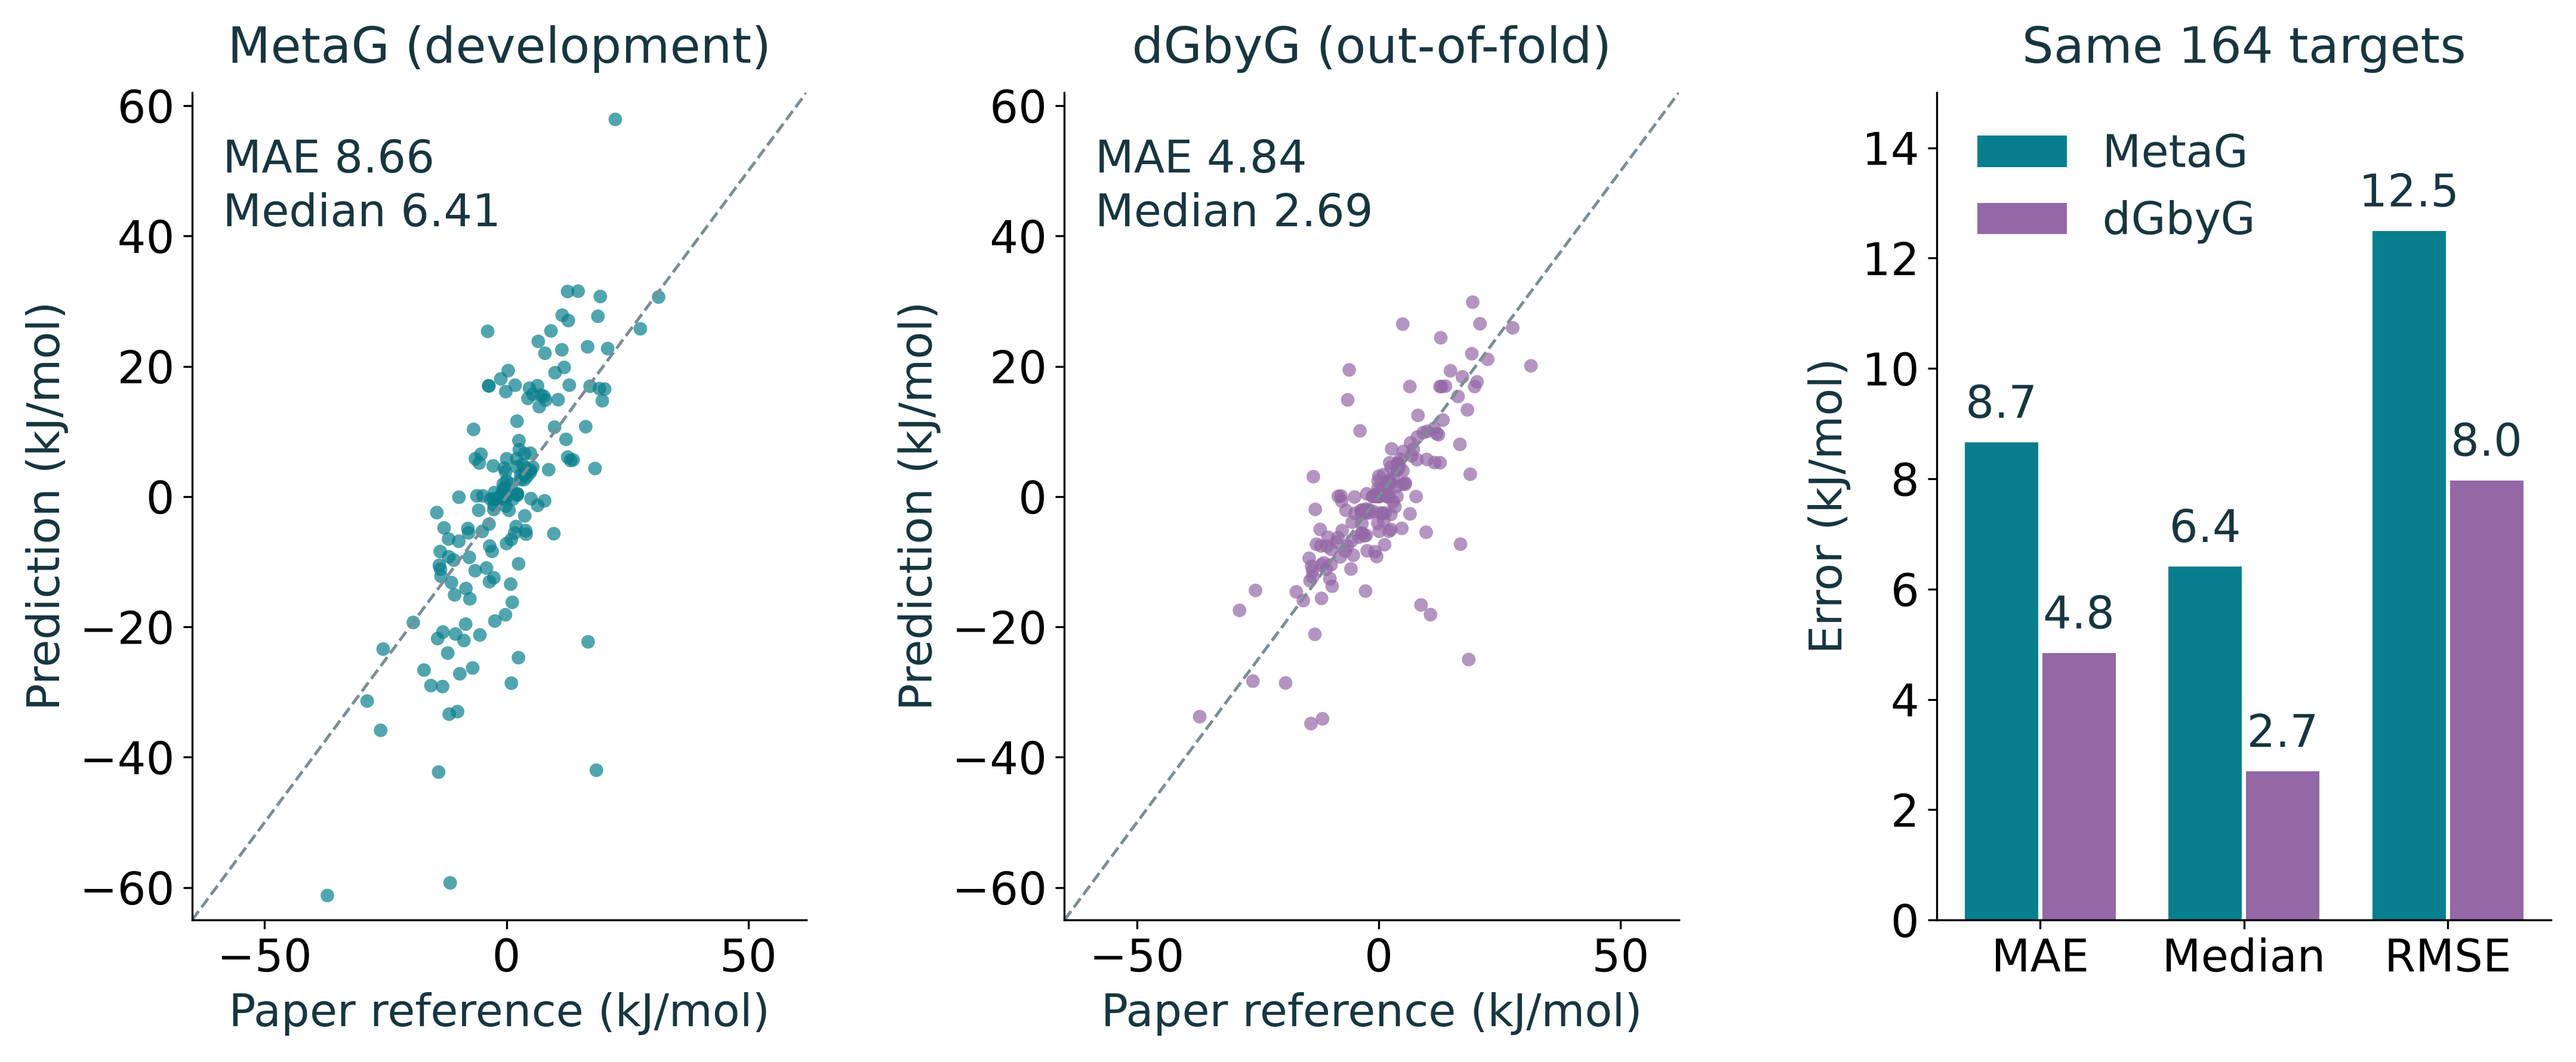
\includegraphics[width=\linewidth,height=4.5cm,keepaspectratio]{matched_dgbyg.png}\par
\small 164 dGbyG-paper targets matched by structure, direction and scale. MetaG bridged from $I=0$ to 0.25 M with eQuilibrator dissociation data.
\messagebox{Held-out dGbyG is more accurate than MetaG here. Only one EC1 reaction is matched.}
\src{artifacts/benchmark/paper\_reproduction/metag\_vs\_dgbyg\_pairs.tsv, metag\_pairing\_audit.tsv. kJ/mol.}
\end{frame}

\begin{frame}{What geometry adds: stereoisomers}
\begin{columns}[c]
\column{.58\textwidth}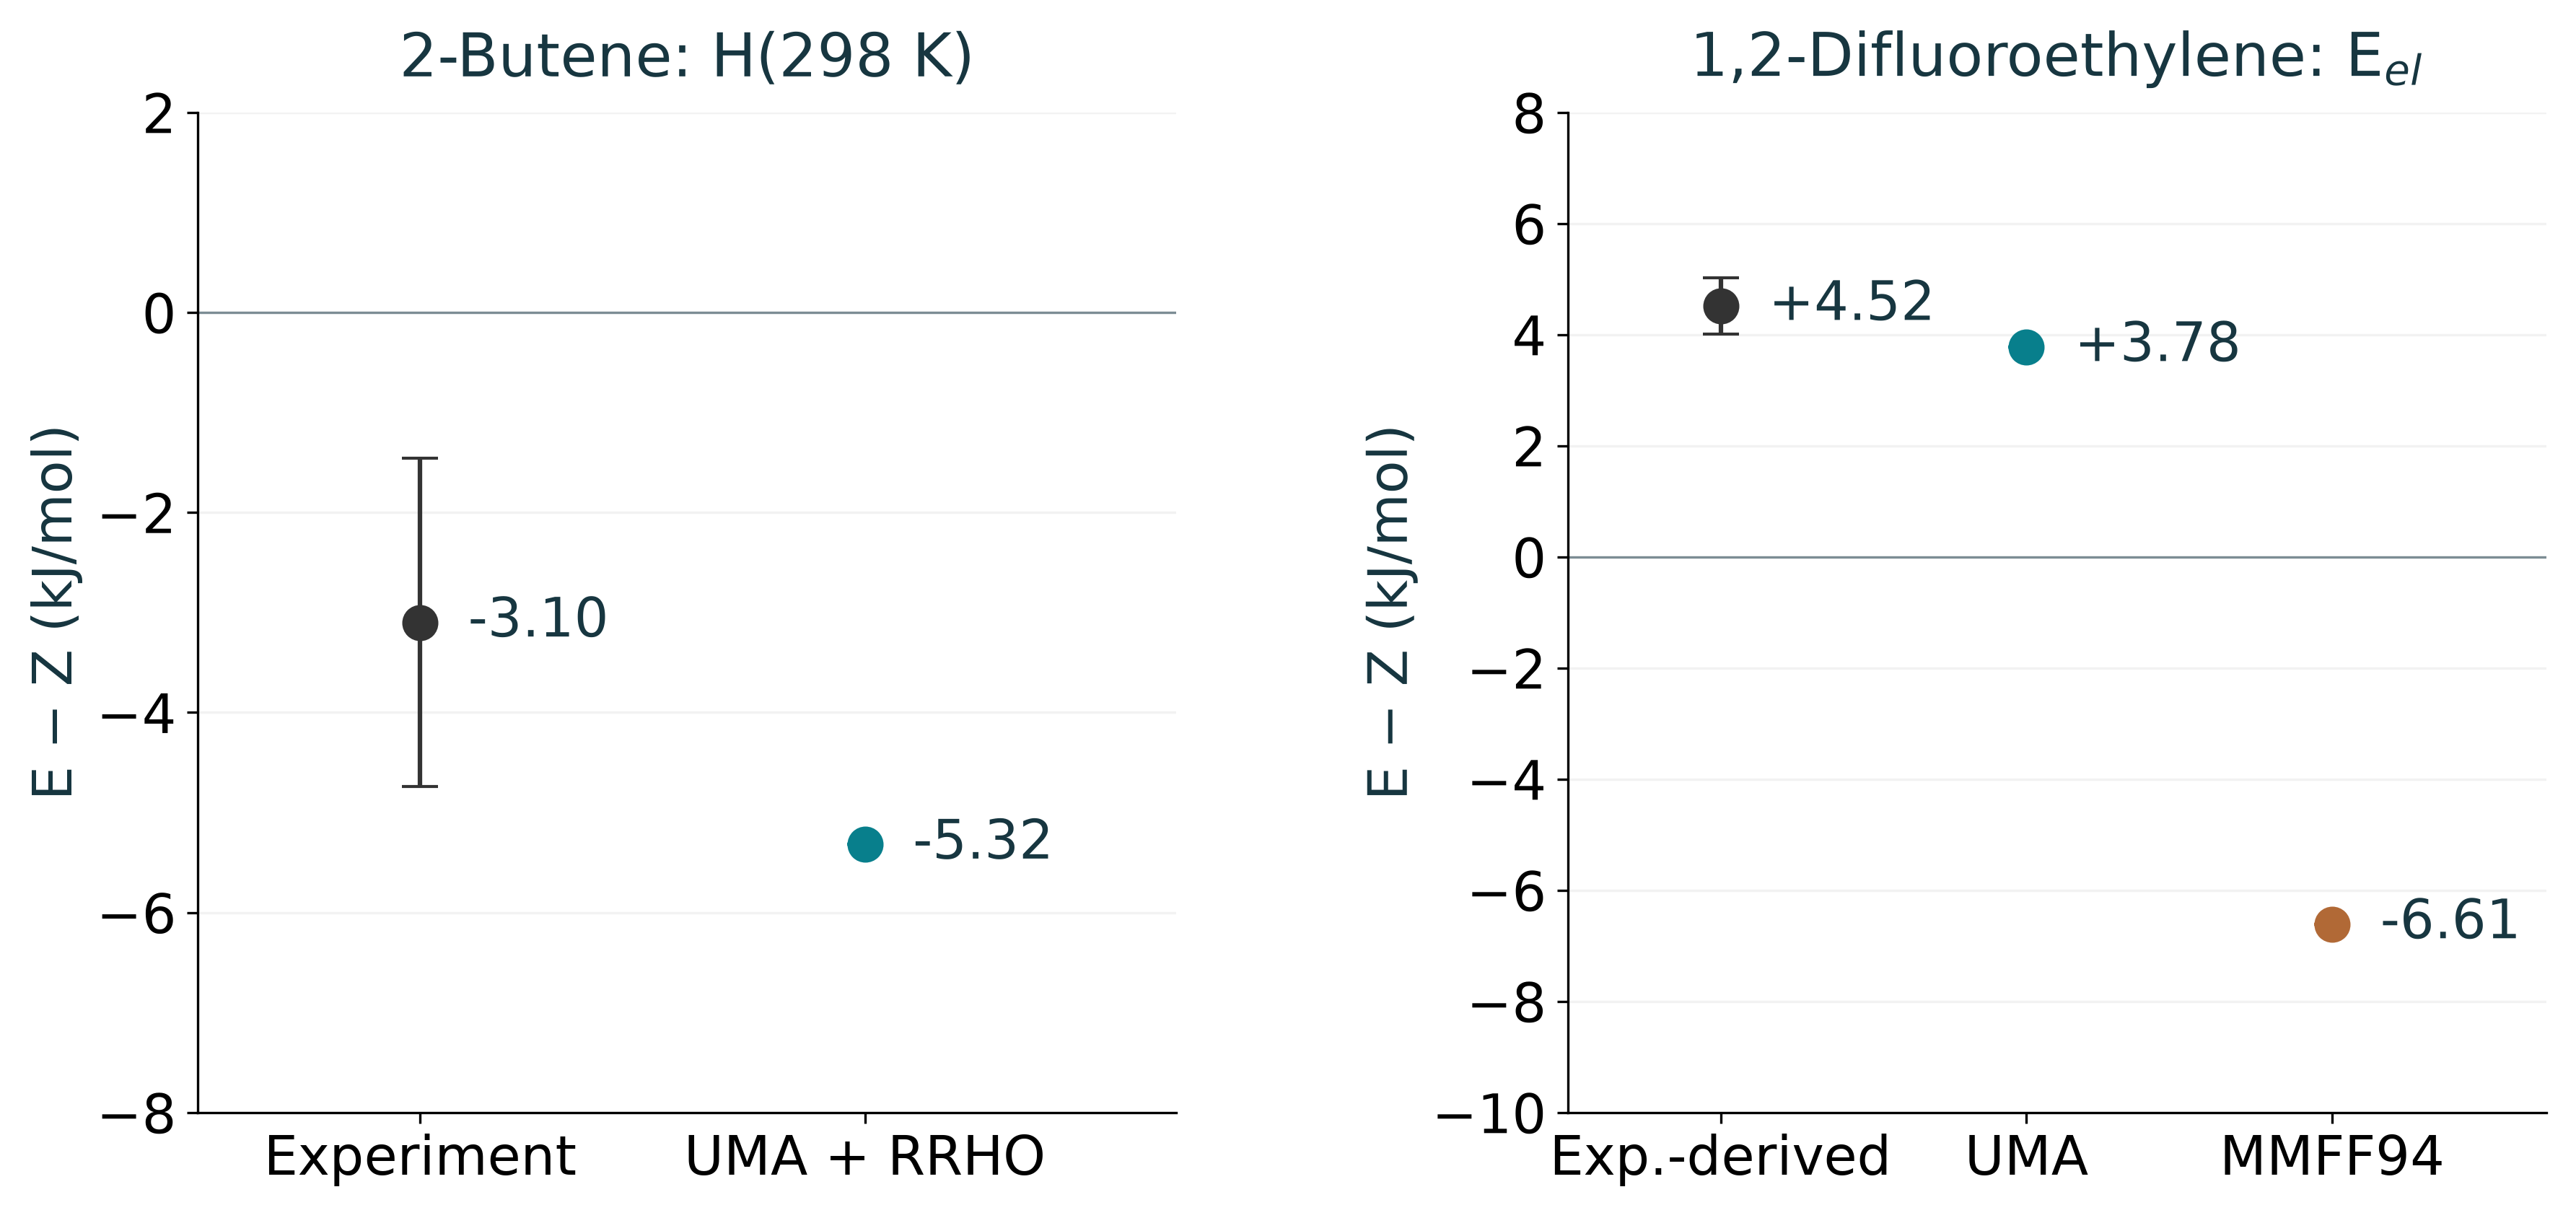
\includegraphics[width=\linewidth,height=4.8cm,keepaspectratio]{stereo_check.png}
\column{.38\textwidth}\small
The published dGbyG encoder gives \textbf{identical inputs} within E/Z and diastereomer pairs (fumarate/maleate; tartrate forms).\par\gap
UMA reproduces the opposite orderings of these two gas-phase pairs; MMFF94 gets difluoroethylene wrong.
\end{columns}
\messagebox{This limits one published encoding, not graph models in general, and is a gas-phase test, not aqueous reaction accuracy.}
\src{state\_qc\_20261007/stereo\_reference\_verified.json; robustness\_20261007/geometry\_probe.tsv. NIST/Prosen 1951; Craig et al. 1971, Table II.}
\end{frame}

\begin{frame}{ModelSEED coverage}
\centering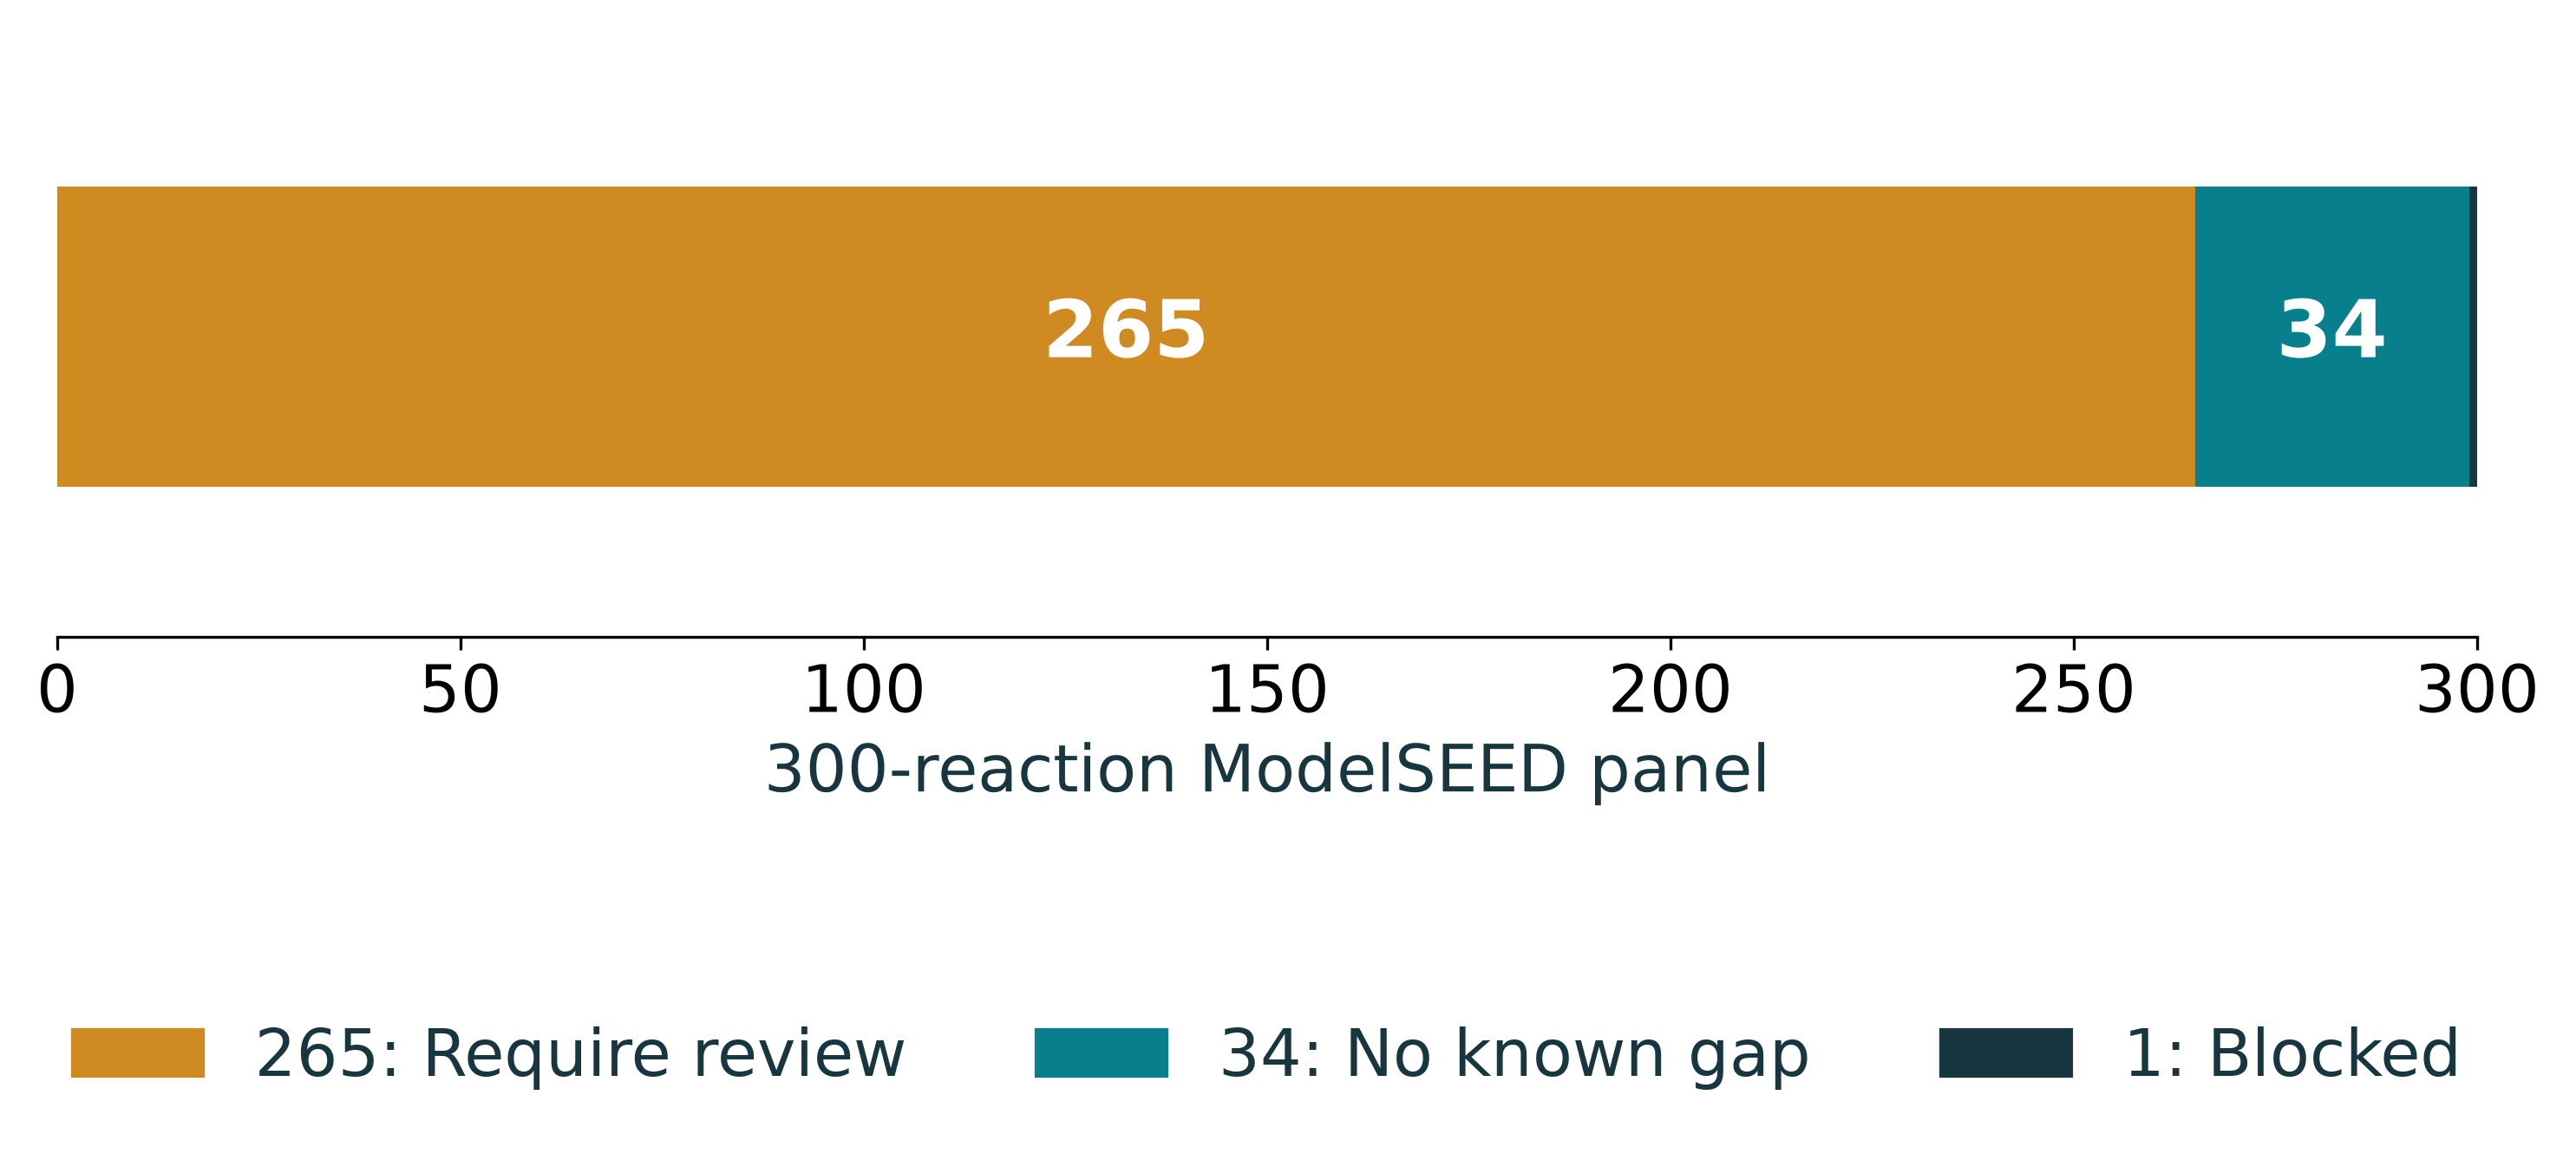
\includegraphics[width=.80\textwidth,height=2.7cm,keepaspectratio]{modelseed_preflight.png}
\begin{columns}[T]
\column{.49\textwidth}\small\textbf{Within 588 unique input structures}\par
238 have multiple acid sites under an independent-site treatment.\par\gap
117 contain aromatic N requiring speciation review.
\column{.47\textwidth}\small\textbf{Interpretation}\par
CPU preflight flags, not counts of wrong predictions. ``No known gap'' is not a guarantee of accuracy. 300-reaction panel, not the full database.
\end{columns}
\src{analysis/code\_review/modelseed\_preflight.json; python -m metag.tools.preflight.}
\end{frame}

\begin{frame}{Summary and limitations}
\begin{columns}[T]
\column{.48\textwidth}\textbf{What MetaG provides}\gap
\begin{itemize}
\item Reaction $\dg$ from UMA energies with no fitted reaction offsets
\item Every term traceable per species and per reaction
\item Explicit failures instead of silent approximations
\item Geometry- and stereo-resolved species energies
\end{itemize}
\column{.48\textwidth}\textbf{Limitations}\gap
\begin{itemize}
\item openTECR MAE 9.54 kJ/mol is a development score
\item Held-out dGbyG is more accurate on matched reactions
\item Independent-site pKa treatment; P--N chemistry withheld
\item Continuum solvation; sampling can miss basins
\item Version 07e awaits a full benchmark and recalibration
\end{itemize}
\end{columns}
\src{Sources as cited on previous slides.}
\end{frame}

% ---------------------------------------------------------------------------
\appendix
\begin{frame}{Appendix: reproducing the dGbyG paper}
\begin{columns}[T]
\column{.47\textwidth}\small
{\footnotesize\setlength{\tabcolsep}{4pt}\begin{tabular}{lrrr}
\toprule
& MAE & Median & RMSE\\\midrule
dGbyG (10-fold) & 9.18 & 4.11 & 25.88\\
eQuilibrator$^*$ (LOO) & 19.46 & 5.33 & 82.88\\
dGPredictor (LOO) & 16.26 & 5.48 & 47.85\\\bottomrule
\end{tabular}}\par\gap
Reconstructed from archived out-of-fold predictions; matches the published headline metrics and all 18 EC-class MAEs.\par\gap
{\scriptsize $^*$ Paper's regression protocol, not today's component-contribution API.}
\column{.49\textwidth}\textbf{Protocol details}\gap
\begin{itemize}\small
\item Headline uses a 675-target historical set, not the 671-target release
\item dGbyG: shuffled 10-fold; baselines: LOOCV on 679 targets
\item Ridge $\alpha$ chosen globally, not nested
\item dGbyG does not win every EC class: EC1 48.7 vs eQuilibrator 38.1
\end{itemize}
\end{columns}
\src{tools/thermo\_benchmark/paper\_reproduction/REPRODUCTION.txt; artifacts/benchmark/paper\_reproduction/. kJ/mol.}
\end{frame}

\begin{frame}{Appendix: reference transformation}
\[
 \dg(c_\star;T)=s[-RT\ln K'_{\rm obs}]
 +\mathcal L_r(c_\star;T)-\mathcal L_r(c_{\rm obs};T)
\]
\begin{itemize}\item $s$ aligns the experimental reaction orientation with ModelSEED.\item $c_\star$: pH 7, $I=0$, pMg 14 (approximately negligible free Mg).\item $\mathcal L_r$ uses dissociation/binding and ionic-strength information; no fitted formation energy enters.\item Temperature remains the measured temperature. Missing $I$ is imputed at 0.25 M and flagged.\end{itemize}
\src{validation/reference\_transform.py; tools/build\_reference.py; eQuilibrator 3.0.}
\end{frame}

\begin{frame}{Appendix: reference curation}
\begin{itemize}
\item Exclude unknown free Mg activity; never substitute total Mg for free Mg
\item Exclude unresolved constant annotations
\item Record source rows and corrections for every retained label
\item 268 retained rows have multiple matching candidates; ambiguity is not proof of a wrong assignment
\end{itemize}
\src{build\_reference.py; reference\_transform.py; curated/reference\_report.json.}
\end{frame}

\begin{frame}{Appendix: protonation partition functions}
For two independent acidic sites relative to a fully protonated reference:
\[
 Z_{\rm independent}=(1+10^{\mathrm{pH}-pK_{a,1}})(1+10^{\mathrm{pH}-pK_{a,2}}).
\]
For two sequential \emph{macroscopic} dissociation constants:
\[
 Z_{\rm sequential}=1+10^{\mathrm{pH}-pK_{a,1}}+
 10^{2\mathrm{pH}-pK_{a,1}-pK_{a,2}}.
\]
The independent product contains an additional term. Production uses the independent form; the sequential form is implemented but not routed.
\src{energetics/protonation.py; eQuilibrator 3.0, DOI: 10.1093/nar/gkab1106; Ullmann, DOI: 10.1021/jp026454v.}
\end{frame}

\begin{frame}{Appendix: code and tests}
\begin{columns}[T]
\column{.49\textwidth}\textbf{Structure}\gap
\begin{itemize}\item CPU-only routing separated from QM\item Pure reaction-energy assembly\item Shared sampling and thermal bookkeeping\item Configuration fingerprint in every result and cache key\end{itemize}
\column{.47\textwidth}\textbf{Not yet in place}\gap
\begin{itemize}\item Immutable per-job configuration\item Dependency identities in cache provenance\item Reliable batch resume and cost accounting\end{itemize}
\end{columns}
\messagebox{387 tests passed, 1 opt-in GPU test skipped (version 07e). This verifies implementation behavior, not predictive accuracy.}
\src{state\_qc\_20261007/tests\_final.log; docs/architecture.md; docs/refactor-status.md.}
\end{frame}

\begin{frame}{Appendix: sources}
\small
\textbf{Local evidence, relative to MetaG\_new}\gap
\begin{itemize}\item \path{artifacts/results/metag_opentecr_calibrated/}\item \path{artifacts/benchmark/comparison/}\item \path{artifacts/benchmark/paper_reproduction/}\item \path{artifacts/benchmark/curated/reference_report.json}\item \path{analysis/code_review/modelseed_preflight.json}\item \path{analysis/state_qc_20261007/}\end{itemize}
\gap
\textbf{External}\par\scriptsize
Fan et al., dGbyG, Cell Systems (2025), DOI: 10.1016/j.cels.2025.101393.\par
\href{https://arxiv.org/abs/2505.08762}{OMol25: quantum-chemical training data and model scope.}\par
\href{https://doi.org/10.1093/nar/gkab1106}{Beber et al., eQuilibrator 3.0.}
\src{Figures are PNG-only. Deck source: slides/MetaG.tex; figure generator: slides/make\_figures.py.}
\end{frame}
\end{document}
